\ifsvnmulti
 \svnkwsave{$RepoFile: xiong/blog/KSe.tex $}
 \svnidlong {$HeadURL: svn://zero.physics.gatech.edu/siminos/xiong/blog/KSe.tex $}
 {$LastChangedDate: 2017-02-15 00:24:45 -0500 (Wed, 15 Feb 2017) $}
 {$LastChangedRevision: 5559 $} {$LastChangedBy: xiong $}
 \svnid{$Id: KSe.tex 5559 2017-02-15 05:24:45Z xiong $}
\fi

\section{\KSe}
\label{sect:KSe}

\PC{2013-03-19 Predrag copied this from \refref{SCD07}, to set up
the conventions for the \KSe\ calculations.}
%
In the formulation
adopted here, the time evolution of the `flame front velocity'
$u=u(x,t)$ on a periodic domain $u(x,t) = u(x+L,t)$ is given by
\beq
  u_t = F(u) = -{\textstyle\frac{1}{2}}(u^2)_x-u_{xx}-u_{xxxx}
    \,,\qquad   x \in [-L/2,L/2]
    \,.
\ee{ks}
Here $t \geq 0$ is the time, and $x$ is the spatial coordinate.
The subscripts $x$ and $t$ denote partial derivatives with respect to
$x$ and $t$. In what follows
we shall state results of all calculations either in units of the
`dimensionless system size' $\tildeL$, or the system size $L = 2 \pi
\tildeL$. All numerical results presented in this report
are for $\tildeL=22/2\pi \simeq 3.5014$.
Spatial periodicity $u(x,t)=u(x+L,t)$
makes it convenient to work in the Fourier space,
\beq
  u(x,t)=\sum_{k=-\infty}^{+\infty} a_k (t) e^{ i k x /\tildeL }
\,,
\ee{eq:ksexp}
with the $1$-dimensional PDE \refeq{ks}
replaced by an infinite set of
ODEs for the complex Fourier coefficients $a_k(t)$:
\beq
\dot{a}_k= \pVeloc_k(a)
     = ( q_k^2 - q_k^4 )\, a_k
    - i \frac{q_k}{2} \sum_{m=-\infty}^{+\infty} a_m a_{k-m}
\,,
\ee{expan}
where $q_k = k/\tildeL$.
Since $u(x,t)$ is real, $a_k=a_{-k}^\ast$, and we can replace the
sum by a $k > 0$ sum.


\begin{description}

\item[2013-06-27 Predrag to \XD] Read the other chapters in this blog,
    study the relevant \KS\ papers\rf{SCD07,Christiansen97}.

\item[2013-07-03 \XD] Here is my first blog post: A question about the
    \KS\ equation. It seems that there are many versions of KS
    equation, and some of them are totally different. The one you used
    in \refref{SCD07}, ``On the {\statesp} geometry of the KS flow in a
    periodic domain'' is \beq
 u_t=-\frac{1}{2}(u^2)_x-u_{xx}-u_{xxxx}
\ee{XD-KSeSCD07}
However, the
equation in \refref{KNSks90}, ``Back in the saddle again: a computer
assisted study of the KS equation'' is:
\beq
 u_t+4\bigtriangleup^2 u
    +\alpha (\bigtriangleup u +\frac{1}{2}(\bigtriangledown u)^2)=0
\ee{XD-KSeSCD07a}
The first order term is different.

\item[2013-07-04 Predrag] That is always annoying when one reads
KS literature - I asked that Evangelos include various transformations
in his thesis, but I cannot find that text, only this:
``The parameter $\alpha$ of \refrefs{KNSks90,ksgreene88} is
related to the system size by $\tildeL=\sqrt{\alpha/4}$.''

In Evangelos
\HREF{../blog/blog.pdf} {blog} we write

``
The {1\dmn} \KSe\ as given in \refrefs{KurTsu75,siv} is (up to overall scaling
factors):
\beq
    y_t=-y_x^2/2-y_{xxxx}-y_{xx}
\,,\qquad       x \in [0,L]
\,,
    \label{eq:KSeOR}
\eeq
with periodic boundary conditions in the $[0,L]$ interval. The form used
here
\beq
    u_t=uu_x-u_{xxxx}-u_{xx}
\,.
    \label{eq:KSeAP}
\eeq
is obtained from \refeq{eq:KSeOR} by differentiating with respect to $x$
and setting \PCedit{$u=-y_x$}.
In study of {1\dmn} \KS\ \eqva\ $x$ in \refrefs{LanThesis,ksgreene88}
is interpreted as ``time", so $y$ is a height of a front,
and $y_x$ its ``velocity".
In the literature  both forms of the equation are
referred to as the \KSe.
''

In Evangelos blog I rescued the text that he did not use in his thesis,
copied below.
Let us know whether this resolves your quandary,
and please do remember to include this in your project
report, so it is available to future students (I should really
include it into an appendix to ChaosBook...)            \toCB

\item[2007-01-20 Evangelos]
Notes on Greene and Kim\rf{ksgreene88}. A copy is in ChaosBook.org/library,
\HREF{http://chaosbook.org/library/index.html}{click here}.

\noindent\textbf{\Eqva\ according to Greene and Kim:}
%
The form of \KSe\ studied by Greene and Kim\rf{ksgreene88} is
\beq
    y_t=-4y_{xxxx}-\alpha\left(y_{xx}+\frac{1}{2}y_x^2
            -\frac{1}{4\pi}\int_0^{2\pi}y_x^2\ dx\right)
\,,\qquad       x \in [0,2\pi]
\,,
    \label{eq:KSeGreeneKim}
\eeq
with  periodic boundary condition on the interval $[0,2\pi]$.
Mean elastic energy density of a spatial profile $y(x,t)$ is defined by
\beq
    E=\frac{1}{2\pi}\int_0^{2\pi}y_x^2\, dx\,.
    \label{KSenergy}
\eeq
% \ES{This definition does not only apply to equilibria. Greene and
% Kim also study the transfer of energy between modes
% in non-stationary trajectories.}.
Taking the derivative of \refeq{eq:KSeGreeneKim}
with respect to $x$ and substituting $y_x=-u$ leads to
\[
    u_t=4u_{xxxx}+\alpha\left(u_{xx}-uu_x\right)
\,.
\]
Rescaling
\beq
    \tilde{x}=\frac{\sqrt{\alpha}}{2} x
\,,\qquad
    \tilde{t}=\frac{\alpha^2}{4} t
\,,\qquad
    \tilde{u}=\frac{2}{\sqrt{\alpha}} u
    \label{eq:GKscale}
\eeq
brings the Greene-Kim equation to the form \refeq{eq:KSeAP} used here.
The dimensionless system size $\tildeL=L/2\pi$ is related to
the Greene-Kim parameter
through $\tildeL=\sqrt{\alpha}/2$.
The system size $L=22$ studied here corresponds to $\alpha=49.0395$.

The ``kinetic energy'' reads in our units:
\PC{shouldn't there be a prefactor $\frac{1}{2}$?}
\beq
    \tilde{E}=\frac{1}{L}\int_0^{L}\tilde{u}^2\, d\tilde{x}\,.
\eeq
Integrating \refeq{ks} in $[0,L]$ we get $c=\tilde{E}$,
since the terms involving $u_x$ and $u_{xxx}$ vanish due to periodicity.
From the scalings \refeq{eq:GKscale} we have $\tilde{E}=\frac{4}{\alpha}E$.


\item[2013-07-03 \XD] In \refref{SCD07} you point out KS equation is
    Galilean invariant: if $u(x,t)$ is a solution, then $u(x-ct)-c$ is
    also a solution. but I am confused, because when I substitute it
    into the equation I get a minus sign. If I change the form to be
    $u(x-ct)+c$, then it is OK.

\item[2013-07-04 Predrag] Thanks for noticing this - you are correct, see
2nd paragraph of Section ChaosBook {\em 26.1.1 Scaling and symmetries.}
(all ChaosBook section and eq.~numbers refer to the stable
\HREF{http://chaosbook.org/version14/pdf.shtml} {version 14} of Dec.
31 2012). The error has propagated from Evangelos
\HREF{http://chaosbook.org/projects/theses.html} {thesis},
{\em section 5.1.2 Symmetries of Kuramoto-Sivashinsky system} to the article.

Embarrassing, but too small an error to change the arXiv version of \refref{SCD07}
(though Evangelos could fix it in his thesis)...

Now I note that the ChaosBook {\em Exercise
26.1.
Galilean invariance of the Kuramoto-Sivashinsky equation} is also in error.
As you are checking the KS papers anyhow, you would help me a lot if you also
checked {\em Chapter 27 Turbulence?} as you went along - that chapter is still
only a draft, has been very hard to write up concisely...
Please correct \refexer{exer-GalInv}, write up the solution
(I'll transfer it back to ChaosBook).                   \toCB
\\{\bf [2013-07-12 \XD] done.}

\item[2013-07-11 \XD] Yesterday I talked with Prof. Predrag and I was
    sceptical about the $1/2$ coefficient in the Fourier transform
    \refeq{expan} of the \KS\ equation \refeq{XD-KSeSCD07}.
\[
 u_t=-\frac{1}{2}(u^2)_x-u_{xx}-u_{xxxx}
 \,.
\]
We perform Fourier transform:
\[
 u(x,t)=\sum_{k=-\infty}^{+\infty} a_{k}(t)e^{ikx/\tilde{L}}
\]
For the nonlinear term $-\frac{1}{2}(u^2)_x$, we get
$-i\frac{q_k}{2}\sum_{m=-\infty}^{+\infty} a_{m}a_{k-m}$,
where $q_k=k/\tilde{L}$. It has the form of
convolution, which comes from one property of Fourier transform.
Now I try to write it down in detail:
\begin{align*}
 -\frac{1}{2}(u^2)_x &=-uu_x \\
 &=-\sum_{m=-\infty}^{+\infty} a_{m}(t)e^{imx/\tilde{L}}
 \sum_{n=-\infty}^{+\infty} \frac{in}{\tilde{L}} a_{n}(t)e^{inx/\tilde{L}}\\
 &=-\sum_{m=-\infty}^{+\infty}\sum_{n=-\infty}^{+\infty} iq_{n} a_{m}(t)e^{iq_{m}x}a_{n}(t)e^{iq_{n}x}\\
 &=-\frac{i}{2}\sum_{m=-\infty}^{+\infty}\sum_{n=-\infty}^{+\infty}
 (q_{n}+q_m) a_{m}(t)e^{iq_{m}x}a_{n}(t)e^{iq_{n}x}\\
 &=-\frac{i}{2}\sum_{m=-\infty}^{+\infty}\sum_{n=-\infty}^{+\infty} q_{n+m} a_{m}(t)a_{n}(t)e^{i(q_{n}+q_m)x}
\end{align*}
If we take out the coefficient of term $e^{iq_{k}x}$, it will give
$-i\frac{q_k}{2}\sum_{m=-\infty}^{+\infty} a_{m}a_{k-m}$, thus the
Fourier transform \refeq{expan} is correct.

\item[2013-07-12 \XD] Wrote up solution to \refexer{exer-GalInv}, {\em
    Galilean invariance of the \KSe.}

\item[2013-07-12 Predrag] Created the research level \refexer{exer-locGalInv},
{\em Local Galilean invariance of \KS.}

\item[2013-06-27 Predrag  to \XD] A discussion of stiffness in
    integrating PDEs can be found
    \HREF{http://www.pvv.ntnu.no/~berland/talks/berland05expintro.pdf}
    {here}. \HREF{http://www.math.ntnu.no/num/expint/} {Here} is Matlab
    package for testing 47 (!) schemes.

Study the methods described in
\HREF{http://www.cns.gatech.edu/~predrag/papers/SCD07.pdf}
{Appendix A} of \refref{SCD07}.
%The authors have lots of experience and they went to the
%    trouble of explaining the best methods they know, so why not read
%    them and implement them?

The plot of what you get for $L=22$
Lyapunov spectrum should confirm the published results (see
{\bf [2009-09-13 Ruslan]} on \refpage{sect:LyapKS},
\reffig{fig:lyapSpecCLG}, \reffig{fig:lyapSpec1},
\reffig{fig:lyapSpec}, and \reftab{tab:ks22shad}) and the
figure\PC{which one? Always state the number} in Kazumasa \etal\
paper\rf{TaGiCh11} (read it
\HREF{http://chaosbook.org/library/KoSa11.pdf} {here}).

\item[2013-06-27 Ruslan]
You can use the method developed by Cox and
Matthews\rf{cox02jcomp} and improved by Kassam and
Trefethen\rf{ks05com}, where the linear part is integrated exactly.
My Matlab code {\tt ksfmetd2.m} is based on this method and it is
stable and reasonably accurate with time step as large as 0.25.  It
also solves variational problem, so can be used to calculate Lyapunov
exponents.  See {\tt ksfmlyap.m} in {\tt siminos/matlab/ruslan/},
read {\tt 00ReadMe.txt}.  If you want to compute Lyapunov exponents
using the standard GS procedure, the relevant code is in {\tt
ksdupo.m} in the same folder (look for the cell "\%\% Compute
Lyapunov exponents of KS (using ksfmlyap and GS)").

\item[2013-06-27 Predrag]
Ruslan uses the same \KSe\ convention as Kassam and
Trefethen\refrefs{ks05com}. I have saved the Trefethen Matlab code
\HREF{http://chaosbook.org/extras/Trefethen/kursiv.m} {here}. Perhaps
you want to c++ it, see how it runs for you, or run it in Matlab and
compare with your code. There might be something else useful on
\HREF{http://chaosbook.org/extras/}{ChaosBook.org/extras} homepage,
for example the simulations by the spring 2007 GaTech chaos class.
You can search the blog for 'Trefethen' for other discussions
(Kazumasa has reservations about the Trefethen\rf{ks05com} algorithm,
but Ruslan is OK with it).
Siminos has other codes, if needed, on a different repository.

\item[2013-01-21 Evangelos] The \KS\ data you need is in \\
\texttt{siminos/matlab/ruslan/kse22orbits.mat},
\\
in a structure called \texttt{eq}.
Eigenvalues are in the field eq.eig and right
eigenvectors are in the field eq.evec. [e.g. eq(k).evec(:,1) is the
eigenvector which corresponds to the first eigenvalue eq(k).eig(1) of
the k'th equilibrium]. However, I have not used the data for a long
time so, it would be better if Ruslan verifies how the Fourier modes
are stored (I think that the numbers in a column vector correspond to
real and imaginary part of the Fourier modes
\[
 (a_1,\, b_1,\, a_2,\, b_2,\, \ldots a_N,\, b_N)
\]
and thus here there are $31+1$ complex Fourier modes (the zero'th mode
is not included)).

In order to get the left eigenvectors you will need to compute the
{\stabmat}.

If you run into problems or have questions please email me so that we
can arrange to talk through Skype.


\item[2013-06-27 Ruslan] To compute {\stabmat} in Matlab, use
\\
\texttt{siminos/matlab/ruslan/ksfm.m}:
\\ {\tt [f, df] = ksfm(0,eq(1).a,22.0)},
\\where {\tt df} will be the {\stabmat} of $EQ_1$.

The idea of the method is described in \refref{SCD07} Appendix A and
B.  The Jacobian matrix is calculated from (B.1) which uses solutions
of (A.4) and (A.6).  Matlab code {\tt ksfmetd2.m} solves (A.4) and
(A.6) simultaneously.  The Jacobian matrix is output in {\tt da}.
You don't need anything else.


\item[2013-07-23 \XD] I don't understand one point of Appendix A in
    paper \rf{SCD07}. After Fourier transform,
\[
 u(x,t)=\sum_{k=0}^{N} a_{k}(t)e^{ikx/\tilde{L}}
\]
we have relation $a_{N-k}^{~}=a_{k}^{*}$ and set $a_0=0$ due to Galilean
invariance, but why can we also set $a_{N/2}=0$ ?
\\
{\bf [2013-07-24 Predrag]} The first relation is due to the reality of
\( u(x,t) \). I suspect that the second one is due to the periodicity
\( u(x,t) = u(x+L,t) \). Let me know if I am wrong?

\item[2013-07-24  \XD] Why both $a_{N/2}=0$ and $a_0=0$? I think
    $a_{N/2}=0$ comes from Galilean invariance of \KS\ equation; while
    we set $a_0=0$ just for the convenience to perform the discrete
    Fourier transform. It is not one component of the Fourier spectrum
    because we are using discrete Fourier transform to truncate the
    nonlinear term in continuous Fourier transform. Am I right?

\item[2013-07-30 Evangelos to \XD] $\dot{a}_0=0$ by Galilean invariance
    and thus $a_0$ is constant. We \emph{choose} this constant to be
    zero so that the mean value of our solutions is zero. Otherwise you
    would get ``drifting solutions.'' $a_{N/2}=0$ is the DFT analog of
    $a_k=a^*_{-k}$, which holds in general for Fourier series of real
    data. (This is discussed in my thesis.)

\item[2013-07-24  \XD] the initial condition of $T_{10.25}$ in
\\*
\texttt{siminos/matlab/ruslan/ks22f90h25t100.mat}
was used in my code. Hoping to get a
periodic graph, I failed. After scrutinizing my code carefully,
I could not find an error, so I suspected that maybe some variables
defined in Ruslan's code were differently
from mine.

I compared my code with \texttt{siminos/matlab/ruslan/ksfmetd2.m},
there is a major difference at the form of the coefficient before the nonlinear term.
Ruslan used \texttt{g = 0.5i*k*N}, but I prefer to \texttt{g=-0.5i*k}.
Such a difference results from the slightly different use of discrete Fourier transform
and the conjugacy of $a_k$, which is \PCedit{$a_{N-k}=a^{*}_k$}.

If we prefer the discrete Fourier transform defined in the Appendix A of
\refref{SCD07},
\[
 u(x,t)=F_N^{-1}[a]_n=\frac{1}{N}\sum_{k=0}^{N-1} a_{k}(t)e^{iq_{k}x_{n}}
\,,
\]
\KS\ equation will be transformed to
\[
 \dot{a_k}=(q_{k}^2-q_k^4)a_k-i\frac{q_k}{2}F_{n}[(F_N^{-1}[a])^2]_k
\,.
\]

Note that the nonlinear term is
\[
-i\frac{q_k}{2}F_{n}[(F_N^{-1}[a])^2]_k=-i\frac{q_k}{2}\frac{1}{N}\sum_{m=-\infty}^{+\infty}a_{m}a_{k-m}
\,.
\]
I think maybe Ruslan hopes the transformed equation is consistent with the form
\[
 \dot{a_k}=(q_{k}^2-q_k^4)a_k-i\frac{q_k}{2}\sum_{m=-\infty}^{+\infty}a_{m}a_{k-m}
\,,
\]
so he keeps the coefficient before the nonlinear term by $N$ times larger.

The sign of the coefficient is defined by whether you treat $\mathbf{a}(t_0)$ as inital condition or
$\mathbf{a}^{*}(t_0)$.


In conclusion, if I insist on my style, I should transform the initial condition $\mathbf{a}(t_0)$
for $T_{10.25}$  to $N\mathbf{a}*(t_0)$, but I think it is better to follow predecessors' style.

\item[2013-07-30 Evangelos to Xiong]
It seems everyone of us uses a different normalization of FFT and sometimes this leads to
confusion. I would suggest that you follow Ruslan's conventions so that you do not need to transform
his data. Also, if you write C++ or Fortran code, I recommend using the excellent FFTW library.




\end{description}

% 2013-11-20 Predrag removed this: \input{../xiong/doc/blog/xcomm.tex}

\subsection{The dimension of \KSe }

\KSe is usually transformed into Fourier space for its benefit of
transforming higher derivatives in the {\statesp} into polynomial terms
in Fourier space. In numerical implementation, we turn to  \xDft  with
truncation number $N$ :  $u_{0}, u_{1}, \cdots, u_{N-1}$.

\[
	\begin{bmatrix}
	a_{0} \\
	a_{1} \\
	\vdots \\
	a_{N-1}
	\end{bmatrix}
	=
	\begin{bmatrix}
	\omega^{0*0} & \omega^{0*1} & \cdots & \omega^{0*(N-1)}\\
	\omega^{1*0} & \omega^{1*1} & \cdots & \omega^{1*(N-1)}\\
	\vdots & \vdots &\ddots & \vdots \\
	\omega^{(N-1)*0} & \omega^{(N-1)*1} & \cdots & \omega^{(N-1)*(N-1)}
	\end{bmatrix}	
	\begin{bmatrix}
	u_{0} \\
	u_{1} \\
	\vdots \\
	u_{N-1}
	\end{bmatrix}
\]

These Fourier modes satisfy $a^{*}_k=a_{N-k} (\mod N)$, which means that
$a_{N/2}$ and $a_{0}$ are both real. This linear transform conserves the freedom
of this system
\[
v_{0},	v_{1},\cdots , v_{N-1} \Rightarrow a_{0}, a_{R,1}, a_{I,1}, \cdots ,
a_{R,N/2-1}, a_{I,N/2-1}, a_{N/2}
\]

Since Floquet multipliers are metric invariant, we can turn to the
Fourier space to calculate the Flouqet multipliers of periodic orbits. At
the same time, the {\cLvs} in the {\statesp} $e^{(i)}_{u}$  and those in
the Fourier space $e^{(i)}_{a}$  satisfy
\[
	e^{(i)}_{a}=M_{i,j}e^{(j)}_{u}
\]

where $M$ is the transforming matrix from $v_{0},	v_{1},\cdots , v_{N-1}$ to \\
$a_{0}, a_{R,1}, a_{I,1}, \cdots , a_{R,N/2-1}, a_{I,N/2-1}, a_{N/2} $.


The flow in the Fourier space is governed by
\begin{equation}
 \dot{a_k}=(q_{k}^2-q_k^4)a_k-i\frac{q_k}{2}F_{N}[(F_N^{-1}[a])^2]_k
 \,.
\end{equation}

In \KS\ system, we set $a_{0}=0$ due to Galilean invariance  and also set  $a_{N/2}=0$ because
$a_{N/2}$ is decoupled from other modes ($q_{N/2} = 0$ for symmetry of the definition of
discrete Fourier Transform), so it decreases rapidly to zero. Therefore, the freedom
of this system is now $N-2$. The flow equation in the tangent space is governed by
\begin{equation}
 \dot{b_k}=(q_{k}^2-q_k^4)b_k-iq_{k} F_{N}[(F_N^{-1}[a])\otimes (F_N^{-1}[b])]_k
 \label{eq:xkstang}
\end{equation}

The initial jacobian matrix in the  \\
$[a_{0}, a_{R,1}, a_{I,1}, \cdots , a_{R,N/2-1}, a_{I,N/2-1}, a_{N/2} ]$ space is  Identity matrix,
which is mapped to $B(0)$ as the initial condition
for equation \ref{eq:xkstang}.
\[B(0)=
\begin{bmatrix}
	0 & 0 & 0 & 0 & \cdots  \\
	1 & 1i & 0 & 0 & \cdots  \\
	0 & 0 & 1 & 1i & \cdots  \\
	\vdots & \vdots  & \vdots &\vdots &\ddots{} \\
	0 & 0 & 1 & -1i & \cdots  \\
	1 & -1i & 0 & 0 & \cdots
\end{bmatrix}
\]

%=======================================================%
\paragraph{Equilibria of \KS\ system at L=22}

I used damped Newton-Raphson method described in \rf{Crofts07thesis} to locate equilibria of
\KSe\ at L=22 and truncation number $N=32$, and I find three equilibria and
calculate their stability exponents. The result is
consistent with that in \refref{SCD07}.

 \begin{figure}[h]
 \centering
 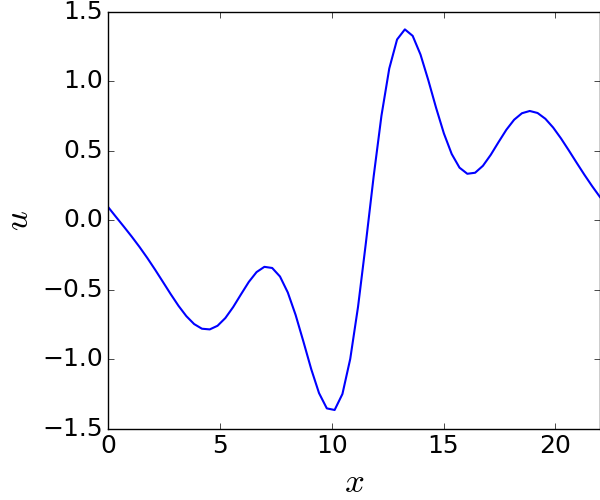
\includegraphics[width=0.3\textwidth]{ksEq1}
 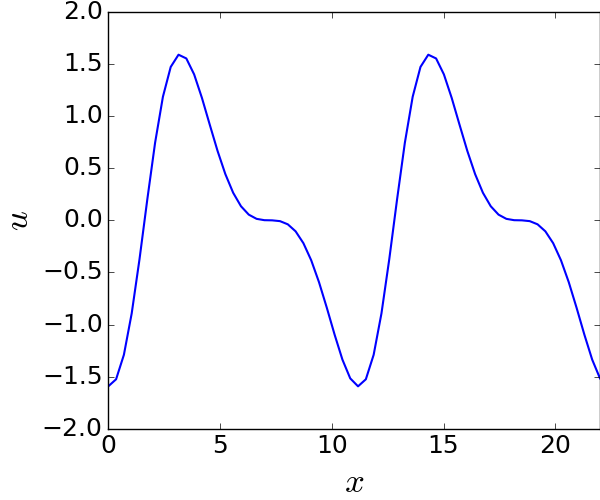
\includegraphics[width=0.3\textwidth]{ksEq2}
 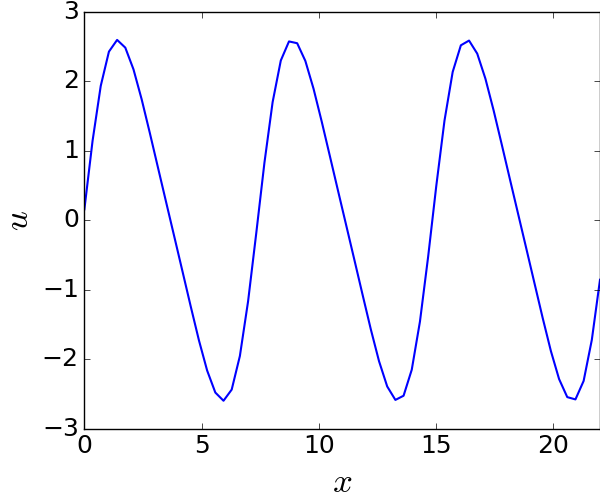
\includegraphics[width=0.3\textwidth]{ksEq3}
 \caption{\Eqva\ solutions in the configuration space.}
 \label{fig:xequi1}
\end{figure}

\begin{figure}[h]
 \centering
 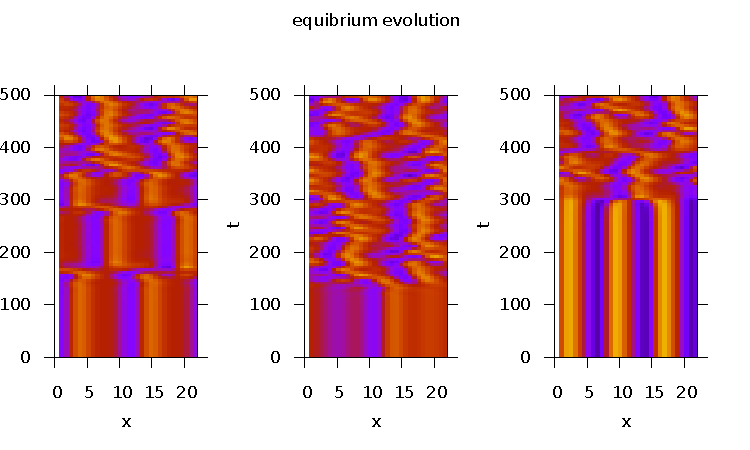
\includegraphics[width=0.8\textwidth]{equi2.pdf}
 \caption{Evolution starting from these \eqva.}
 \label{fig:xequi2}
\end{figure}

\refFig{fig:xequi1} is not as smooth as that in \rf{SCD07} and the magnitude of the waves has different
scales and phases. The underlining reason for the difference is that
 we have slightly different definitions of \xDft and  these equilibria exhibit  translational invariance.

 \refFig{fig:xequi2} is the evolution of these equilibria. Since they are unstable, the states turn to be
 chaotic after about 100 time units for the first two equilibria, while the third one stays about 300 time units
 before collapse.



 For equilibria, the {\stabmat} is constant $A(x_{eq})$; so is the jacobian matrix
 $J^{t}(x_{eq})=\exp(A(x_{eq})t)$.
 Therefore, the stability exponents are just the eigenvalues of $A(x_{eq})$ and the {\cLvs}
 are just the eigenvectors of $A(x_{eq})$.  The stability exponents  are exactly the same with those documented in
 \rf{SCD07} , here I only post my result for $E_{3}$ equilibrium.
 \\
   0.09335 + 0.00000i \\
   0.09334 + 0.00000i \\
  -0.00000 + 0.00000i  \\
  -0.41277 + 0.00000i\\
  -0.61075 + 0.37587i\\
  -0.61075 - 0.37587i \\
  -0.61075 + 0.37588i \\
  -0.61075 - 0.37588i \\
  -1.66413 + 0.00000i \\
  -1.66413 + 0.00000i \\

The other two sets of exponents are saved in \\
\texttt{/siminos/xiong/matlab/equilibria}.


\paragraph{Relative equilibria}
Relative equilibrium is defined as $u(x,t) = u(x-ct)$,
which means $f_{k}(a) = v_{k}(a) +icq_{k}a_{k}$. The second term  $cq_{1}t(a)$
is a vector in group tangent direction
in $\mathbb{U}(1)$ space. In order to implement Newton's method, we need to get the
explicit form of $f'_{k}$:
\begin{equation}
  \begin{bmatrix}
    A + cq_{1}\mathbf{T} & q_1  t(a) \\
    t(a) & 0
  \end{bmatrix}
  \cdot
  \begin{bmatrix}
    \Delta b_1 \\
    \Delta c_1 \\
    \vdots \\
    \Delta c_{N/2-1}
  \end{bmatrix}
  =
  \begin{bmatrix}
    f_{1,R} \\
    f_{1,I} \\
    \vdots \\
    f_{N/2-1,I}\\
  \end{bmatrix}
  \,.
  \label{eq:relativeeq}
\end{equation}
$\mathbf{T}$ is the generator of SO(2), and $A$ is the {\stabmat}
in the full state space. The last row in \ref{eq:relativeeq} comes from the
constraint $t(a)\cdot \Delta a = 0$. For \KS\ system with $L=22$, only two
relative equilibria
are found. Note that equation \ref{eq:relativeeq} is also capable
detecting equilibria ($c = 0$). Relative equilibrium is moving on the
group orbit $x(t)=g(-ctq_1)x(0)$, and the relation of {\stabmat}
at different points on this group orbit is simple.
$A(x)\delta x = \delta v(x)$ and $A(gx)\delta(gx)=\delta v(gx)$ infer
$A(gx)g\delta x = g\delta v(x)$, which is $A(gx)g=gA(x)$, so the
eigenvectors of $A$
at point $x$ and $g(-ctq_1)x$ are related by group transformation
$g(-ctq_1)$; however, this vector is not covariant along the group
trajectory. since $J^{\delta t}v=(1+A\delta t)v = (1+\lambda\delta t) v$,
which is not in the same direction as
$g(\delta \theta)v = v+\delta\theta \mathbf{T}v$. According to
Chaosbook, The correct {\stabmat} in this case is
$A+cq_1\mathbf{T}$.

The reasoning behind is every simple. Let's consider a general case:
$x(t)=g(ct)x(0)$. The Jacobian is decomposed as
\[
J^{\zeit} = J^{\Delta t} (x_n) J^{\Delta t} (x_{n-1})\cdots  J^{\Delta t} (x_1)
\,,
\]
where $\Delta t = t/n$ and $x_{k}=g[c(k-1)\Delta t] x_1$. Since
$J(gx)=gJ(x)g^{-1}$, we have
\begin{align*}
J^{\zeit} & = g[c(n-1)\Delta t]J^{\Delta t} (x_1)g^{-1}[c(k-1)\Delta t]
\cdots J^{\Delta t} (x_1) \\
& = [g(-c\Delta t)J^{\Delta t} (x_1)]^{n} \\
& \approx [1 - c\Delta t \mathbf{T} + \Delta t A]^n \\
& \to e^{(-c\mathbf{T}+A)\zeit}
\end{align*}
Here, $\zeit$ denotes the period of the \reqv. Therefore,
$A-c\mathbf{T}$ is the {\stabmat} for relative equilibria.

 %==========================================================%
\subsection{Symmetry of \KSe }
\label{subsect: symkse}

One-dimensional \KSe\  $u_t=-\frac{1}{2}(u^2)_x-u_{xx}-u_{xxxx}\,,x\in [0,L]$ on a
periodic domain ($L=22$) has three different
symmetry:
\begin{itemize}
\item Galilean invariance. if $u(x,t)$ is a solution, then
  $u(x-ct,t)+c$ is also a solution, where c is a constant
  number. These two solutions have different mean velocity
  $\int dx\, u$.
\item Reflection symmetry.  $Ru(x,t)=-u(-x,t)$ is also a solution
  if $u(x,t)$ is a solution.
\item transitional invariance. $\tau_{l/L}u(x,t)=u(x+l,t)$.
\end{itemize}

Numerically, \KSe\
could be transformed into
Fourier space by discrete Fourier transform with truncation
to $N=32$ or $N=64$.
\[
a_{k}(t)=\sum_{n=0}^{N-1}u(x_{n},t)e^{iq_{k}x_{n}},\quad
u(x_{n},t)=\sum_{k=0}^{N-1}a_{k}(t)e^{iq_{k}x_{n}}
\,.
\]
In this way, dynamics in Fourier space is governed by
\[
\dot{a_k}=(q_{k}^2-q_k^4)a_k-i\frac{q_k}{2}F_{N}[(F_N^{-1}[a])^2]_k
\,,
\]
where $q_k = 2\pi k/L$, and the coefficients are complex
$a_{k}=b_{k}+ic_{k}$.


Since $u(x,t)$ is real, $a_{k}(t)=a^{*}_{N-k}(t)$; thus only half of the
Fourier modes are independent. The zero mode $a_{0}$ denotes the
mean velocity of a solution and $\dot{a}_{0}=0$
 enables eliminating Galilean invariance by
setting $a_{0}=0$.
Also after setting $a_{N/2}=0$ \cite{SCD07}, the number of independent variables is $N-2$,
\begin{equation}
\label{eq:fourierspace}
[b_{1},c_{1},b_{2},c_{2},\cdots,b_{N/2-1},c_{N/2-1}]
\,,
\end{equation}
which is the Fourier state space in the discussion that follows.
On the other hand, reflection and translation invariance in
configuration space corresponds to  equivariance of
 \eqref{eq:fourierspace} under group operation
 $R=diag(-1,1,-1,1,\cdots)$ and  $g(l)=diag(r_{1},r_{2},\cdots,r_{N/2-1})$,
where
\[
r_{k}=
\begin{pmatrix}
  \cos(q_{k}l) & \sin(q_{k}l) \\
  -\sin(q_{k}l) & \cos(q_{k}l)
\end{pmatrix}
,\quad k=1,2,\cdots,N/2-1
\,.
\]

 Since periodic orbits of \KS\ system
are time invariant and equivariant under \SOn{2}\ group transformation
 $g(l)$, there should be two marginal exponents which corresponds
to the velocity field $v(x)$ and group tangent $t(x)=\mathbf{T}x$
respectively, where
$\mathbf{T}$ is the generator of \SOn{2}\ rotation:
\[
\mathbf{T}=diag(t_{1},t_{2},\cdots,t_{N/2-1}),\quad
t_{k}=
\begin{pmatrix}
  0 & q_{k} \\
  -q_{k} & 0
\end{pmatrix}
\,.
\]

Especially, for covariant vectors of pre-periodic orbits.
The Jacobian is defined as $J_{p}=RJ^{T_{p}}$, where $T_{p}$ is the prime
period. The two marginal Floquet vectors $v(x)$ and $t(x)$ have
opposite  Floquet multipliers, namely 1 and -1, that is why \ped\ could tell
them and their corresponding Floquet vectors apart. The prof is very
straightforwards.
\begin{align*}
  J_{p}v(x(0))& = RJ^{T_{p}}v(x(0)) \\
  & = Rv(x(t_{p})) =Rv(Rx(0)) \\
  & =R\cdot R v(x(0)) \\
  & =v(x(0))
\end{align*}

\begin{align*}
  J_{p}t(x(0))&= RJ^{T_{p}}t(x(0)) \\
  & = Rt(x(T_{p})) =Rt(Rx(0)) \\
  & = R\mathbf{T}Rx(0) \\
  & = -\mathbf{T}x(0)=t(x(0))\\
\end{align*}

In the last step, we have use the anti-commutation relation
$R\mathbf{T}=-\mathbf{T}R$ which can be verified easily. Therefore,
the velocity field has positive Floquet multiplier 1 and group
tangent has negative Floquet multiplier -1. In table
\ref{tab:FloqExpPPO1}, we can see the third Floquet vector is
the velocity field while the fourth Floquet vector is the group tangent.

%%%%%%%%%%%%%%%%%%%%%%%%%%%%%%%%%%%%%%%%%%%%
\subsection{\On{2}\ factorization of {\Fd} for \KSe }

\KSe\ is invariant under \On{2}\ symmetry, which joins \SOn{2}\ rotations
with $\Dn{1}=\{e,R\}$ reflections. The expected way of writing down the
symmetry reduced trace formula in this case is referring to
the character table of \On{2}, but could we first quotient out
\SOn{2}\ symmetry in the trace formula and then further discuss the
behavior under reflection $R$, like the one-dimensional map
example
invariant under reflection in the Chaosbook ?

The first problem arising in this procedure is the convergence
of \SOn{2}\ reduced trace formula. According to the argument in
Chaosbook,
\begin{align*}
  \sum_{\beta=0,m=0}^{\infty}\frac{1}{s-s_{m,\beta}}
  = & \sum_{m=-\infty}^{\infty}d_{m} \sum_p T_{p}\sum_{r=1}^{\infty}
    \chi_{m}( g_p^r)
{
 e^{r (\beta A_{p}-sT_{p})}
  \over
 {\left|\det\!\left(1-\tilde{M}_{p}^r\right)\right|}
} \\
    = & \sum_{m=-\infty}^{\infty} \sum_p T_{p}\sum_{r=1}^{\infty} e^{-imr\theta_{p}}
{
 e^{r (\beta A_{p}-sT_{p})}
  \over
 {\left|\det\!\left(1-\tilde{M}_{p}^r\right)\right|}
}
\,,
\end{align*}
where $\theta_{p}$ is the group parameter of $g_{p}$ and $m$ is the
index of non-equivalent irreducible representations.
The second identity rises from the fact that the non-equivalent
irreducible representations of \SOn{2}\ are all one-dimensional:
$e^{-im\phi}$. Here,
\[
\sum_{m=-\infty}^{\infty}e^{-imr\theta_{p}}=
\int dx \sum_{m=-\infty}^{\infty}\delta(x-mr)e^{-i\theta_{p} x}
\]
the Fourier transform of a Dirac Comb. I
don't know how to evaluate this formula. On the other hand,
the trace of {\evOper} is defined as
$\mathcal{L}^{t}(y,x)=\int dx \delta(x-f^{t}(x))$, I don't know
why relative periodic orbits will contribute because they
never close.

\begin{description}

\item[2014-04-24 Xiong Ding]
I found the frequently referred to \refref{Creagh91}, ``Semiclassical
trace formulas in the presence of continuous symmetries'' which is
focused one the trace formula for quantum systems. I don't know whether
it deserves reading because it will take me some time to understand it.
Any opinion?

\item[2014-04-27 Predrag] If I credit a paper, you should try to read it
at some point - it is important to read the literature yourself, and blog
your notes here, I might have missed something important when I read it.
You know this from the periodic Schur decomposition. I try to only credit
papers that are actually relevant to our work. Creagh papers are good.
But you are already doing the right stuff to derive the classical trace
formula, so you do not need to read it urgently.

I will not answer your questions above, because from our conversation
today it looks like you have figured out the derivation.

\item[2014-05-02 Xiong Ding] I had a hard time going through the
argument about
\[
{\cal L}_{ba} (y,x) = D(h)_{ba} {\cal L} (y,x)
\]\noindent
as the starting point to understand discrete factorization. For me,
the projection approach is easier to grasp. Projection
operator is defined as
\[
P_\alpha = \frac{d_\alpha}{|G|} \sum_{h\LieEl\in\Group} \chi_\alpha (h) {\bf h}^{-1}
\]
for a discrete symmetry group
$G=\{{ e},{ g}_2,\ldots,{ g}_{|G|}\}$. The orthogonality and completeness
of projection operator
can be easily verified by the orthogonality relation among characters of
irreducible representation. Define $ \cal L_\alpha=P_\alpha \cal L$, then
the trace of {\evOper} $\cal L$ can be decomposed into a sum of
$ \sum_\alpha \tr {\cal L}_\alpha$ because of the completeness of projection
operators.
\Xiong{2014-05-03}{Here the decomposition of trace just relies on the
completeness of projection operators, we haven't used the commutation
relation between {\evOper} and group transform. Am I right?}
So we only need to investigate the projected trace formula:
\begin{align*}
\tr {\cal L}_\alpha & = \frac{d_\alpha}{|G|}\sum_{h \LieEl\in\Group} \chi_\alpha (h)
{\bf h}^{-1} \int_\pS dx \, {\cal L} ( x,x) \\
& =\frac{d_\alpha}{|G|}\sum_{h \LieEl\in\Group} \chi_\alpha (h) {\bf h}^{-1}
\sum_{a \LieEl\in\Group}\int_{\tilde{\pS}} d(a\tilde{x}) \,{\cal L} (a\tilde{x},a\tilde{x})
\\
& =\frac{d_\alpha}{|G|}\sum_{h \LieEl\in\Group} \chi_\alpha (h) {\bf h}^{-1}\,\cdot
|G|\int_{\tilde{\pS}} d(\tilde{x}) \,{\cal L} (\tilde{x},\tilde{x}) \\
& = d_\alpha \sum_{h \LieEl\in\Group} \chi_\alpha (h) \int_{\tilde{\pS}} d\tilde{x} \,
{\cal L} ({\bf h}^{-1} \tilde{x},\tilde{x})
\end{align*}
In the above derivation, we have used the invariance of {\evOper}
under group transform. For a periodic orbit in the fundamental domain
$\tilde{p}$, we follow the standard argument in Chaosbook and get
\[
\int_{\tilde{\pS}} d\tilde{x} \, {\cal L} ({\bf h}^{-1} \tilde{x},\tilde{x}) =
\cl{\tilde{p}} \sum_{r=1}^\infty { e^{r \beta \cdot \Obser_{\tilde{p}}}
\over  | \det \left( {\bf 1}- {\tilde\monodromy}_{\tilde{p}}^{r} \right)
| } \delta_{n,\cl{\tilde{p}} r}\delta_{h,h_{\tilde{p}}^r}
    \,;
\]
so, the {\Fd} is
\bea
F(z) &=& \prod_\alpha F_\alpha (z)^{d_\alpha}
    \continue   %\,\, , \quad \quad
F_\alpha (z) &=&
{\rm exp}  \left( - {
         \sum_{\tilde{p}} \sum_{r=1}^\infty {1 \over r}
 {\chi_\alpha (h_{\tilde{p}}^r)  z^{\cl{\tilde{p}} r}
e^{r \beta \cdot \Obser_{\tilde{p}}}
 % {\phi_p^r}
 \over  | \det \left( {\bf 1}- {\tilde\monodromy}_{\tilde{p}}^{r} \right) | }
         } \right)
\,\,  ,
\eea
which is discrete factorization for maps. The same method can be applied to
flows with discrete symmetry:
\[
F_\alpha (z) =
{\rm exp}  \left( - {
         \sum_{\tilde{p}} \sum_{r=1}^\infty {1 \over r}
 {\chi_\alpha (h_{\tilde{p}}^r) e^{r (\beta \cdot \Obser_{\tilde{p}}-sT_{\tilde{p}})}
 % {\phi_p^r}
 \over  | \det \left( {\bf 1}- {\tilde\monodromy}_{\tilde{p}}^{r} \right) | }
         } \right)
\]

Making an approximation
$| \det \left( {\bf 1}- {\tilde\monodromy}_{\tilde{p}}^{r} \right) | \approx
|\Lambda_{\tilde{p}}|$ where $\Lambda_{\tilde{p}}$ is the product of all
expanding multipliers, we get the factorized zeta function:
\begin{equation}
F_\alpha (z) =
{\rm exp}  \left( -
         \sum_{\tilde{p}} \sum_{r=1}^\infty {1 \over r}
 \chi_\alpha (h_{\tilde{p}}^r) t_{\tilde{p}}^{r} \right)
\label{eq:redzeta}
\end{equation}

Formula \eqref{eq:redzeta} is the ultimate goal of Discrete Factorization,
which basically tells us that,
equipped with character table of the group in question, we can write down
all the factorized zeta function for all classes of this group. On the
other hand, in order to verify our result,
let's calculate the zeta
function in the full state space.
\begin{align*}
  F(z) &= \prod_\alpha F_\alpha (z)^{d_\alpha} \\
  &= {\rm exp}  \left( -
    \sum_{\tilde{p}} \sum_{r=1}^\infty {1 \over r}\sum_{\alpha}
    \left(d_{\alpha}\chi_\alpha (h_{\tilde{p}}^r)\right) t_{\tilde{p}}^{r} \right) \\
  &= {\rm exp}  \left( -
    \sum_{\tilde{p}} \sum_{r=1}^\infty {1 \over r}
    |G|\delta_{h_{\tilde{p}}^{r},e}  t_{\tilde{p}}^{r} \right) \\
  &= {\rm exp}  \left( -
    \sum_{\tilde{p}} \sum_{k=1}^\infty {|G| \over mk}
     t_{\tilde{p}}^{mk} \right)
     \,,
\end{align*}
that is
\begin{equation}
  \label{eq:fullzeta}
  F(z)= \left(1-t_{\tilde{p}}^{\frac{|G|}{m}}\right)^{m} \,,
\end{equation}
where $m$ is the smallest positive number such that $h_{\tilde{p}}^{m}=e$, namely
the multiplicity of the periodic orbit in the full state space.
Formula \eqref{eq:fullzeta} is just the left side of
\beq
(1-t_{\tilde{p}}^{h_p})^{g/h_p}
=\det \left(1- D(h_{\tilde p}) t_{\tilde p} \right)
=
\prod_{\alpha} \det(1-D_{\alpha}(h_{\tilde{p}}) t_{\tilde{p}} )^{d_\alpha}
\eeq
in Chaosbook and actually formula \eqref{eq:redzeta} is the right side of
it. For completeness, I derive their equivalence here. By the
definition of character and representation of a group,
$\chi_\alpha (h_{\tilde{p}}^r)= \tr D_{\alpha}(h_{\tilde{p}}^r)
=\tr (D_{\alpha}(h_{\tilde{p}}))^{r}$ where $D$ is the regular representation
of this group, so \eqref{eq:redzeta} can be rewritten as follows,
\begin{align*}
F_\alpha (z) & =
{\rm exp}  \left( -
  \tr \sum_{\tilde{p}} \sum_{r=1}^\infty {1 \over r}
 (D_{\alpha}(h_{\tilde{p}}))^{r} t_{\tilde{p}}^{r} \right) \\
& ={\rm exp}  \left(
  \tr \sum_{\tilde{p}} \ln (1-D_{\alpha}(h_{\tilde{p}}))
  \right) \\
& = \prod_{\tilde{p}} \det(1-D_{\alpha}(h_{\tilde{p}}))
\end{align*}
Here, we have used relation $\tr \ln= \ln \det$. All calculation of
factorized zeta function in Chaosbook is conducted by
$\det(1-D_{\alpha}(h_{\tilde{p}}))$, but I are apt to use \eqref{eq:redzeta}
because it doesn't contain information about any specific representation.
\Xiong{2014-05-05}{I am not sure whether I understand it correctly here.}
All the following examples are analyzed by \eqref{eq:redzeta}.

{\bf [2015-06-20 Predrag]} moved the $C_{n}$ character table to
siminos/xiong/thesis/chapters/symm.tex .

\paragraph{$C_{n}$} case

When $h_{\tilde p}=e$,
\[
F_{A}=F_{\Gamma_j}={\rm exp} (-\sum_{r=1}^\infty {1 \over r}t_{\tilde{p}}^{r} )
=1-t_{\tilde p}
\,,
\]
Where we only investigate the contribution from one specific periodic
orbit and ignore the summation $ \sum_{\tilde{p}}$.

When $h_{\tilde p}=C_n^k$, Similarly,
\[
F_{A}=1-t_{\tilde p}
\]
\[
F_{\Gamma_j}={\rm exp} (-\sum_{r=1}^\infty {1 \over r}e^{\frac{i2\pi kjr}{n}}
t_{\tilde{p}}^{r} )
=1-e^{\frac{i2\pi kj}{n}} t_{\tilde p}
\,,
\]
In sum,
\vskip 12pt
\begin{tabular}{rlccc}

$h_{\tilde p}$ &  & &  $A$  &  $\Gamma_{j}$ \\
$e$:
& $(1-t_{\tilde p} )^n$  &=&$(1-t_{\tilde p})$ & $(1-t_{\tilde p})$  \\
$C_n^{k}$:
& $(1-t_{\tilde p}^m )^{\frac{n}{n}}$ &=&  $(1-t_{\tilde p})$ & $(1-\exp(\frac{i2\pi kj}{n})t_{\tilde p})$ \\
\end{tabular}
\vskip 12pt
\noindent

{\bf [2015-06-20 Predrag]} moved the $D_{n}$ character tables to
siminos/xiong/thesis/chapters/symm.tex .

\paragraph{$C_{nv}$ ($n$ odd)} case:
When $h_{\tilde p}=e$,
\[
F_{A_1}=F_{A_2}={\rm exp} (-\sum_{r=1}^\infty {1 \over r}t_{\tilde{p}}^{r} )
=1-t_{\tilde p}
\]
\[
F_{E_j}={\rm exp} (-\sum_{r=1}^\infty {2 \over r}t_{\tilde{p}}^{r} )
=(1-t_{\tilde p})^2
\]
When $h_{\tilde p}=C_n^k$, the same goes for $A_1$ and $A_2$:
$F_{A_1}=F_{A_2}=1-t_{\tilde p}$, but for $E_j$, it requires a little
special treatment.
\begin{align*}
F_{E_j}= & {\rm exp} (-\sum_{r=1}^\infty {1 \over r}2\cos\frac{2\pi kjr}{n}
t_{\tilde{p}}^{r} ) \\
= & {\rm exp} \left(-\sum_{r=1}^\infty {1 \over r}(\exp(\frac{i2\pi
kjr}{n})+\exp(-\frac{i2\pi kjr}{n}))t_{\tilde{p}}^{r} \right) \\
= & \left(1-\exp(\frac{i2\pi kj}{n})t_{\tilde p} \right)
\left(1-\exp(-\frac{i2\pi kj}{n})t_{\tilde p} \right) \\
= & 1-2\cos\frac{2\pi kj}{n}t_{\tilde p}+t_{\tilde p}^2
\end{align*}
When $h_{\tilde p}\in \{\sigma,C_n^1\sigma,\cdots,C_n^{n-1}\sigma\}$,
$h_{\tilde p}^2=e$.
\begin{align*}
F_{A_1}= &1-t_{\tilde p} \\
F_{A_2}= &{\rm exp} (-\sum_{r=even}^\infty {1 \over r}t_{\tilde{p}}^{r}
+\sum_{r=odd}^\infty {1 \over r}t_{\tilde{p}}^{r} )
=(1+t_{\tilde p}) \\
F_{E_j}= &{\rm exp} (-\sum_{r=even}^\infty {1 \over r}2t_{\tilde{p}}^{r})
=(1-t_{\tilde p}^2)
\end{align*}

In sum,

\vskip 12pt
\begin{tabular}{rlcccc}

$h_{\tilde p}$ &  & &  $A_1$  &  $A_2$  &  $E_j$  \\
$e$:
& $(1-t_{\tilde p} )^{2n}$  &=&$(1-t_{\tilde p})$ & $(1-t_{\tilde p})$ &
$ (1-t_{\tilde p})^4 $ \\
$C_n^k,C_n^{n-k} $:
& $(1-t_{\tilde p}^m )^{\frac{2n}{m}}$ &=&  $(1-t_{\tilde p})$ & $(1-t_{\tilde p})$ &
$ (1-2\cos(\frac{2\pi kj}{n})t_{\tilde p}+t^{2}_{\tilde p})^2 $ \\
$\sigma,C_n^1\sigma,\cdots,C_n^{n-1}\sigma$:
& $(1-t_{\tilde p}^2 )^{n}$ &=&  $(1-t_{\tilde p})$ &                      $(1+t_{\tilde p})$ &$ (1-t_{\tilde p}^2)^2 $ \\
\end{tabular}
\vskip 12pt
\noindent

{\bf [2015-06-20 Predrag]} moved the $D_{n}$ character tables to
siminos/xiong/thesis/chapters/symm.tex .

\paragraph{$C_{nv}$ ($n$ even)} case:
%When $h_{\tilde p}=e$, we have $F_{A_1}= %F_{A_2}=F_{B_1}=F_{B_2}=1-t_{\tilde p}$
%and $F_{E_j}=(1-t_{\tilde p})^2$
%
%When $h_{\tilde p}=C_2$, similarly, $F_{A_1}= F_{A_2}=1-t_{\tilde p}$,
%$F_{B_1}=F_{B_2}=1-(-1)^{n/2}t_{\tilde p}$ and
%$F_{E_j}=(1-(-1)^jt_{\tilde p})^2$.

Similar calculation gives us the following
factorized zeta function table.

\vskip 12pt
\begin{center}
\begin{tabular}{b{1cm}lcccccl}

$h_{\tilde p}$ &  & &  $A_1$  &  $A_2$  &  $B_1$  &  $B_2$  &  $E_{j}$  \\
$e$:
& $(1-t_{\tilde p} )^{2n}$  &=&$(1-t_{\tilde p})$ & $(1-t_{\tilde p})$ &
                        $(1-t_{\tilde p})$ &$(1-t_{\tilde p})$&$ (1-t_{\tilde
 p})^4 $ \\
$C_2$:
& $(1-t_{\tilde p}^2 )^n$ &=&  $(1-t_{\tilde p})$ & $(1-t_{\tilde p})$ &
$(1-(-1)^{\frac{n}{2}}t_{\tilde p})$ &$(1-(-1)^{\frac{n}{2}}t_{\tilde p})$ &
$(1-(-1)^jt_{\tilde p})^4 $ \\
$C_n^{k}$ (odd):
& $(1-t_{\tilde p}^m )^{\frac{2n}{m}}$ &=&  $(1-t_{\tilde p})$ & $(1-t_{\tilde p})$ &
$(1+t_{\tilde p})$ &$(1+t_{\tilde p})$ &
$ (1-2\cos(\frac{2\pi kj}{n})t_{\tilde p}+t^{2}_{\tilde p})^2 $ \\
$C_n^{k}$ (even):
& $(1-t_{\tilde p}^m )^{\frac{2n}{m}}$ &=&  $(1-t_{\tilde p})$ & $(1-t_{\tilde p})$ &
$(1-t_{\tilde p})$ &$(1-t_{\tilde p})$ &
$ (1-2\cos(\frac{2\pi kj}{n})t_{\tilde p}+t^{2}_{\tilde p})^2 $ \\
$\sigma$:
& $(1-t_{\tilde p}^2 )^n$&=& $(1-t_{\tilde p})$ & $(1+t_{\tilde p})$ &
$(1-t_{\tilde p})$ &$(1+t_{\tilde p})$& $ (1-t_{\tilde p}^2)^2 $ \\
$C_n^1\sigma$:
& $(1-t_{\tilde p}^2 )^n$&=& $(1-t_{\tilde p})$ & $(1+t_{\tilde p})$ &
$(1+t_{\tilde p})$ &$(1-t_{\tilde p})$& $ (1-t_{\tilde p}^2)^2 $ \\
\end{tabular}
\end{center}
\vskip 12pt
\noindent

When it comes to continuous symmetry, projection operator is
\beq
 {P}_\eigenvG
 = d_\eigenvG \int_{G} dg\,
   \, \chi_\eigenvG(g^{-1})  O_g
\,.
\eeq
The corresponding trace formula in the irreducible subspace is
\beq
    \sum_{\beta=0}^\infty
    {1 \over \eigenvL -\eigenvL_{\eigenvG,\beta} }
    =
     d_\eigenvG \sum_p
 \period{p}
    \sum_{r=1}^\infty
 \chi_\eigenvG( g_p^r)
{
 e^{r (\beta \Obser_p -\eigenvL\period{p})}
  \over
 {\left|\det\!\left(\matId-
\tilde{\monodromy}_{\eigenvG,p}^r\right)\right|}
}
\,.
\eeq
Therefore the spectral determinant is factorized as

\bea
 \det(\eigenvL - \Aop) &=& \prod_\alpha F_\alpha (z)^{d_\alpha}
    \continue   %\,\, , \quad \quad
F_\alpha (z) &=&
{\rm exp}  \left( - {
         \sum_{\tilde{p}} \sum_{r=1}^\infty {1 \over r}
 {\chi_\alpha (g_{\tilde{p}}^r)  z^{\cl{\tilde{p}} r}
e^{r \beta \cdot \Obser_{\tilde{p}}}
 % {\phi_p^r}
 \over  | \det \left( {\bf 1}- {\tilde\monodromy}_{\tilde{p}}^{r} \right) | }
         } \right)
\,\,
\eea
It differs from the discrete case on that now the group operator
$g_{\tilde{p}}$ is continuous and the factorization may have infinite terms.

\paragraph{SO(2)} As the limit of $C_n$ when $n$ goes to infinity,
the irreducible representation of SO(2) is also one dimensional, but now
it has infinite number of representations labeled by $j$ in the following
character table.
\vskip .3cm
\begin{center}
\begin{tabular}{c|cr}
$SO(2)$       & $A$& $\Gamma_{j}$ \\
\hline
$  e  $        &   1  &   1   \\
$C(\phi)$      &   1  &  $\exp(ij\phi)$  \\
\end{tabular}
\end{center}
\vskip .3cm
\noindent
Here $\phi\in[-\pi,\pi)$ is the parameter of this group and
$j=\cdots,-2,-1,1,2,\cdots$. The corresponding
factorized zeta functions are obtained in the same way as $C_n$.
However, I don't what to put in the $?$ positions in the table follows.

\vskip 12pt
\begin{tabular}{rlccc}

$h_{\tilde p}$ &  & &  $A$  &  $\Gamma_{j}$   \\
$e$:
& ?  &=&$(1-t_{\tilde p})$ & $(1-t_{\tilde p})$  \\
$C(\phi_{p})$:
& ? &=&  $(1-t_{\tilde p})$ & $(1-\exp(ij\phi_{p})t_{\tilde p})$  \\
\end{tabular}
\vskip 12pt
\noindent
In this case,
\[
\det(\eigenvL - \Aop)=
{\rm exp}  \left( - {
         \sum_{\tilde{p}} \sum_{r=1}^\infty {1 \over r}
         \sum_{j=-\infty}^{\infty}e^{ijr\phi_{\tilde{p}}}
 {  z^{\cl{\tilde{p}} r}
e^{r \beta \cdot \Obser_{\tilde{p}}}
 % {\phi_p^r}
 \over  | \det \left( {\bf 1}- {\tilde\monodromy}_{\tilde{p}}^{r} \right) | }
         } \right)
\]
Since $\sum_{j=-\infty}^{\infty}e^{ijr\phi_{\tilde{p}}}=2\pi\delta(r\phi_{\tilde{p}})$,
and $\phi_{\tilde{p}}$ can not divide $2\pi$,
it seems that relative periodic orbits do not contribute to
{\Fd} in this case. That is what I am confused on.
\Xiong{2014-05-05}{ Prof. Predrag suggested me reading materials about
regularization. I tried, but cannot understand the math.}

\paragraph{O(2)} As the limit of $C_{nv}$ when $n$ goes to infinity,
$O(2)=\{e,C(\phi),\sigma,C(\phi)\sigma\}$ with $\phi\in (0,2\pi)$.
It has two one dimensional irreducible representations ($A_1$ and $A_2$)
and infinite two dimensional irreducible representations.
The character table and factorized zeta functions can be computed in
the same way as follows.

\vskip .3cm
\begin{center}
\begin{tabular}{c|crr}
$O(2)$       & $A_1$& $A_2$&  $E_{j}$ \\
\hline
$  e  $        &   1  &   1   &  2  \\
$C(\phi)  $        &   1  &   1  & $2\cos(j\phi)$  \\
$\sigma,C(\phi)\sigma$ &   1  &  -1  &  0
\end{tabular}
\end{center}
\vskip .3cm
\noindent

\vskip 12pt
\begin{tabular}{rlcccl}

$h_{\tilde p}$ &  & &  $A_1$  &  $A_2$  &  $E_j$  \\
$e$:
& ?  &=&$(1-t_{\tilde p})$ & $(1-t_{\tilde p})$ &
$ (1-t_{\tilde p})^4 $ \\
$C(\theta_{p})$:
& ? &=&  $(1-t_{\tilde p})$ & $(1-t_{\tilde p})$ &
$ (1-2\cos(j\theta_{p})t_{\tilde p}+t^{2}_{\tilde p})^2 $ \\
$\sigma$:
& ? &=& $(1-t_{\tilde p})$ & $(1+t_{\tilde p})$ &
$ (1-t_{\tilde p}^2)^2 $ \\
\end{tabular}
\vskip 12pt
\noindent

I don't know how to deal with the infinite summation in this case either.


\item[2014-05-05 Xiong Ding] Here I list several formulas used in the
above post.

\begin{equation}
\frac{1}{2\pi}\sum_{n=-\infty}^{\infty}e^{inx} = \delta(x)
\end{equation}
This identity comes from one definition of delta function
$\delta(x)=\lim_{N\to \infty}
\frac{1}{2\pi}\frac{\sin(N+1/2)x}{\sin(\frac{1}{2}x)}$ and simple
calculation gives
$\sum_{n=-N}^{N}e^{inx}=\frac{\sin(N+1/2)x}{\sin(\frac{1}{2}x)}$.

\begin{equation}
\sum_{R}\chi_\alpha(R) \chi_\beta(SR^{-1})=\frac{|G|}{d_\alpha}\,
\delta _{\alpha,\beta} \chi_\alpha(S)
\end{equation}
This is the orthogonality between characters of irreducible
representations. If we set $S=e$, then it reduces to
$\sum_{R}\chi_\alpha(R) \chi_\beta(R^{-1})=|G|\delta _{\alpha,\beta}$.
The orthogonality of projection operators can be checked:
\begin{align*}
  P_\alpha P_\beta = & \frac{d_\alpha}{|G|}\, \frac{d_\beta}{|G|}
  \sum_{h,s\LieEl\in\Group} \chi_\alpha (h) \chi_\alpha (s) {\bf h}^{-1} {\bf s}^{-1} \\
  = & \frac{d_\alpha}{|G|}\, \frac{d_\beta}{|G|} \sum_{s\LieEl\in\Group}
  \frac{|G|}{d_\alpha}\,\delta _{\alpha,\beta} \chi_\alpha(sh)(\bf{sh})^{-1} \\
  = &\delta _{\alpha,\beta} \frac{d_\alpha}{|G|}\,\sum_{s\LieEl\in\Group}
  \chi_\alpha(s){\bf s}^{-1} \\
  = & \delta _{\alpha,\beta}\, P_\alpha
\end{align*}

The last formula is
\begin{equation}
\sum_\alpha d_\alpha \chi_\alpha (R) = |G|\, \delta_{e,R}
\label{eq:groupcomplete}
\end{equation}
which comes from orthogonality relation above. For regular representation,
the trace of $R$ in terms of irreducible representations is
$\chi (R)=\sum_\alpha a_\alpha \chi_\alpha (R)$, so the summation of all group
elements gives
\[
\sum_{R}\chi (R)\chi_\alpha (R^{-1})=\sum_\alpha a_\alpha \sum_{R}
\chi_\alpha (R) \chi_\alpha (R^{-1}) =|G|\, a_\alpha
\]
On the other hand, $\chi (R)=|G|\, \delta_{e,R}$ for regular representation,
then the left side of the above expression is just $|G|\,\chi_\alpha (e)$,
so $a_\alpha =\chi_\alpha (e) =d_\alpha $ the dimension of $\alpha_{th}$
irreducible representation. In this way, we obtain \refeq{eq:groupcomplete}.
Now the completeness of projection operator can be checked:
\[
\sum_\alpha P_\alpha = \sum_\alpha \frac{d_\alpha}{|G|} \sum_{h\LieEl\in\Group}
  \chi_\alpha (h)  {\bf h}^{-1}
 =\frac{1}{|G|} \sum_{h\LieEl\in\Group} \left(\sum_\alpha d_\alpha \chi_\alpha (h)
   \right){\bf h}^{-1}
=e
\]


\end{description}
